\chapter{数据库设计}
\section{数据库环境说明}
本系统的数据系统采用MySQL数据库系统。


\section{数据库的命名规则}

\indent    1.名称的命名方式选用头字母大写(头分法)\\
\indent    2.允许单词缩写,很长的单词可以采取前几个字母作为代表\\
\indent    比如广告活动Advertisements缩写为Ads\\
\indent    3.属性名基本采用驼峰命令法的方式\\
\indent    比如用户名"user name"表示为userName \\
\indent    4.表名是复数,首字符大写\\
\indent    5.字段不带类型前缀


\section{逻辑设计}
\begin{figure}[H]
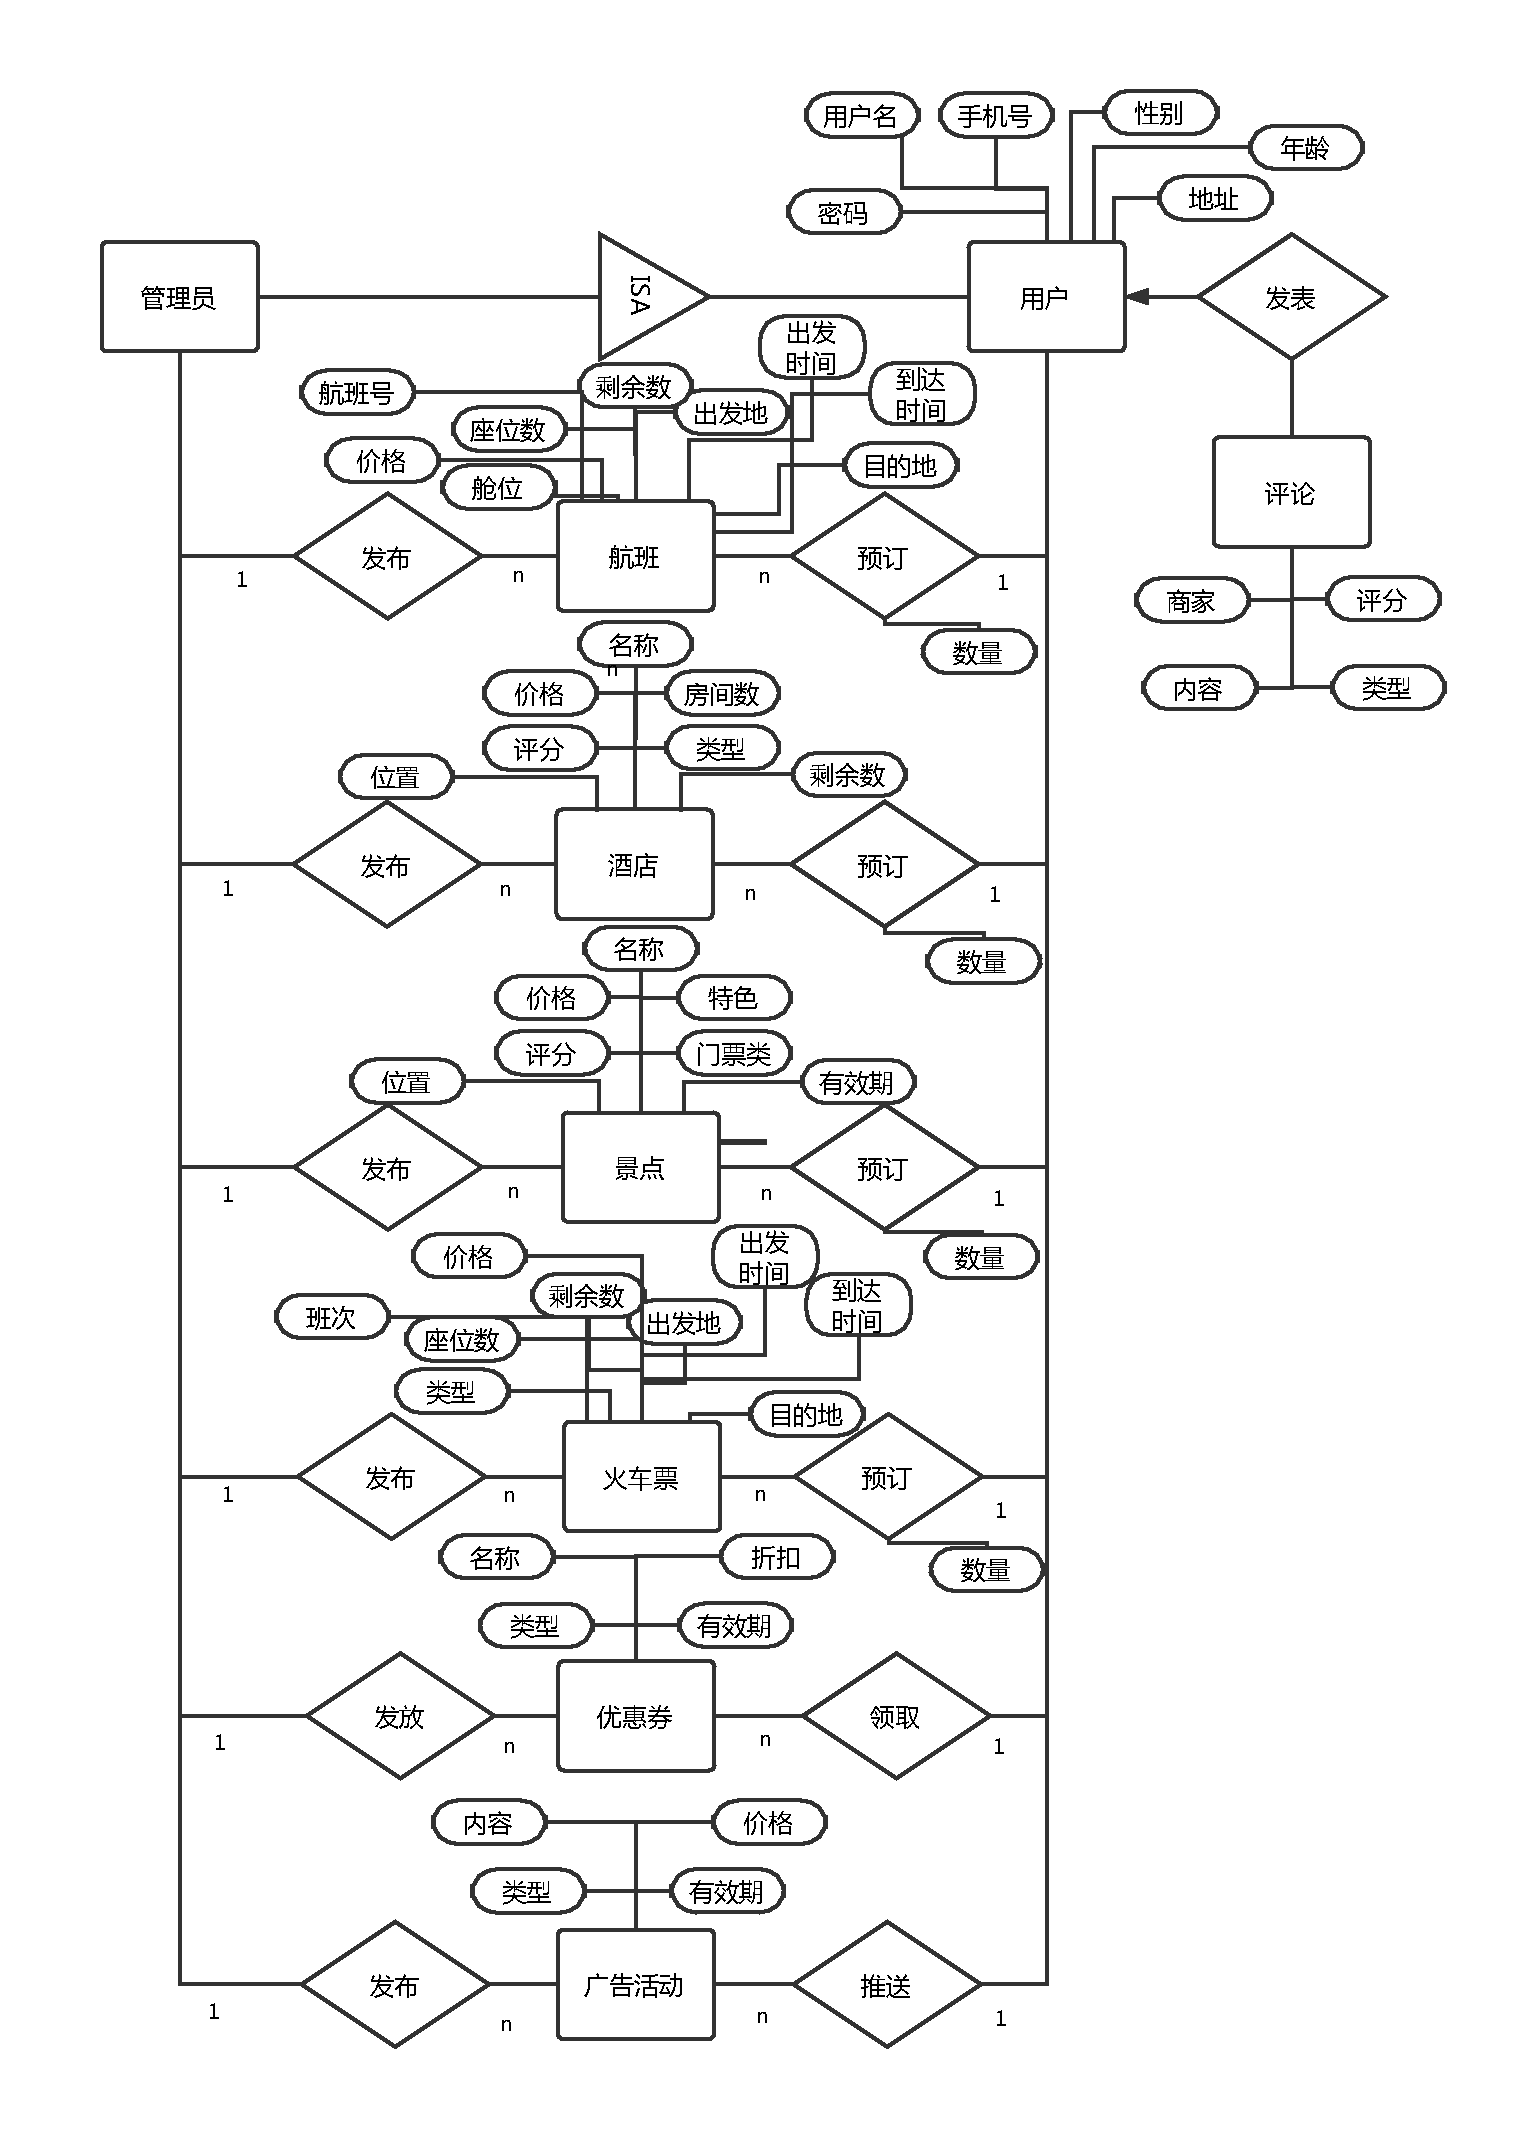
\includegraphics[width=16cm]{db}
\caption{逻辑设计图} \label{fig:figure1}
\end{figure}

\section{物理设计}
\subsection{数据库产品}
瑞典MySQL AB公司的MySQL数据库,非分布式。
\subsection{实体属性、类型、精度}
\subsubsection{活动数据表设计}
\begin{table}[H]
\centering
\caption{活动数据表Ads设计} \label{tab:order-database}
\begin{tabular}{|c|c|c|c|c|}
    \hline
    字段名 & 类型 & 大小 & 说明 & 备注 \\
    \hline
    id & integer & 64 & 活动的唯一标识符 & 主键\\
    \hline
    adName & char & 256 & 活动的名称 &  \\
    \hline
    adContent & char & 1024 & 活动的内容 & \\
    \hline
    adPrice & integer & 64 & 活动的价格 & \\
    \hline
    endTime & dateTime & 256 & 活动的截止时间 & \\
    \hline
\end{tabular}
\note{活动数据表Ads设计}
\end{table}

\subsubsection{客户数据表设计}
\begin{table}[H]
\centering
\caption{用户数据表Users设计} \label{tab:client-database}
\begin{tabular}{|c|c|c|c|c|}
    \hline
    字段名 & 类型 & 大小 & 说明 & 备注 \\
    \hline
    id & integer & 64 & 用户的唯一标识符 & 主键\\
    \hline
    userName & char & 128 & 用户的用户名 & Unique唯一 \\
    \hline
    passWd & char & 256 & 用户的登录密码 & \\
    \hline
    custName & char & 128 & 用户的姓名 & \\
    \hline
    custSex & char & 32 & 用户的性别 & \\
    \hline
    custAge & integer & 64 & 用户的年龄 & 大于0 \\
    \hline
    custPhone & char & 128 & 用户的手机号 & \\
    \hline
    custAddr & char & 512 & 用户的地址 & \\
    \hline
\end{tabular}
\note{用户数据表Users设计}
\end{table}



\subsubsection{优惠券数据表设计}
\begin{table}[H]
\centering
\caption{优惠券数据表Coupons设计} \label{tab:order-database}
\begin{tabular}{|c|c|c|c|c|}
    \hline
    字段名 & 类型 & 大小 & 说明 & 备注 \\
    \hline
    id & integer & 64 & 优惠券的唯一标识符 & 主键\\
    \hline
    couponName & char & 256 & 优惠券的名称 &  \\
    \hline
    couponType & char & 64 & 优惠券类型(比如酒店/航班等) & \\
    \hline
    couponRate & integer & 64 & 优惠券的折扣 & 范围在1~99\\
    \hline
    endTime & dateTime & 256 & 优惠券使用的截止时间 & \\
    \hline
\end{tabular}
\note{优惠券数据表Coupons设计}
\end{table}


\subsubsection{用户评论数据表设计}
\begin{table}[H]
\centering
\caption{用户评论数据表Marks设计} \label{tab:order-database}
\begin{tabular}{|c|c|c|c|c|}
    \hline
    字段名 & 类型 & 大小 & 说明 & 备注 \\
    \hline
    id & integer & 64 & 评论的唯一标识符 & 主键\\
    \hline
    userName & char & 128 & 评论者的用户名 & 外码,来自Customers表 \\
    \hline
    markScore & float & 64 & 用户评分 & \\
    \hline
    markContent & char & 1024 & 评论内容 & \\
    \hline
    markName & char & 256 & 被评论的商家名 & \\
    \hline
    markType & char & 128 & 评论类型 & \\
    \hline
\end{tabular}
\note{用户评论数据表Marks设计}
\end{table}


\subsubsection{航班数据表设计}
\begin{table}[H]
\centering
\caption{航班数据表Flights设计} \label{tab:order-database}
\begin{tabular}{|c|c|c|c|c|}
    \hline
    字段名 & 类型 & 大小 & 说明 & 备注 \\
    \hline
    id & Integer & 64 & 飞机票的唯一标识符 & 主键\\
    \hline
    flightId & char & 128 & 航班号 &  \\
    \hline
    seatType & char & 64 & 舱位 & \\
    \hline
    price & integer & 64 & 飞机票价格 & 大于0 \\
    \hline
    seatNum & integer & 64 & 座位数目 & 大于0 \\
    \hline
    avaiNum & integer & 64 & 剩余座位数 & >= 0 \\
    \hline
    fromCity & char & 256 & 出发城市 & \\
    \hline
    arivCity & char & 256 & 到达城市 & \\
    \hline
    fromTime & datetime & 256 & 起飞时间 & \\
    \hline
    arivTime & datetime & 256 & 到达时间 & \\
    \hline
\end{tabular}
\note{航班数据表Flights设计}
\end{table}


\subsubsection{火车票数据表设计}
\begin{table}[H]
\centering
\caption{火车票数据表Trains设计} \label{tab:order-database}
\begin{tabular}{|c|c|c|c|c|}
    \hline
    字段名 & 类型 & 大小 & 说明 & 备注 \\
    \hline
    id & Integer & 64 & 火车票的唯一标识符 & 主键\\
    \hline
    trainId & char & 128 & 列车班次 &  \\
    \hline
    seatType & char & 64 & 座位类型 & \\
    \hline
    price & integer & 64 & 火车票价格 & 大于0 \\
    \hline
    seatNum & integer & 64 & 座位数目 & 大于0 \\
    \hline
    avaiNum & integer & 64 & 剩余座位数 & >= 0 \\
    \hline
    fromCity & char & 256 & 出发城市 & \\
    \hline
    arivCity & char & 256 & 到达城市 & \\
    \hline
    fromTime & datetime & 256 & 出发时间 & \\
    \hline
    arivTime & datetime & 256 & 到达时间 & \\
    \hline
\end{tabular}
\note{火车票数据表Flights设计}
\end{table}


\subsubsection{酒店数据表设计}
\begin{table}[H]
\centering
\caption{酒店数据表Hotels设计} \label{tab:order-database}
\begin{tabular}{|c|c|c|c|c|}
    \hline
    字段名 & 类型 & 大小 & 说明 & 备注 \\
    \hline
    id & Integer & 64 & 酒店预订记录的唯一标识符 & 主键\\
    \hline
    hotelName & char & 256 & 酒店名称 &  \\
    \hline
    hotelLoca & char & 512 & 酒店位置 & \\
    \hline
    hotelScore & float & 64 & 酒店评分 & \\
    \hline
    roomType & char & 64 & 房间类型 & \\
    \hline
    price & integer & 64 & 价格 & 大于0 \\
    \hline
    roomNum & integer & 64 & 房间数目 & 大于0 \\
    \hline
    avaiNum & integer & 64 & 剩余房间数 & >=0 \\
    \hline
\end{tabular}
\note{酒店数据表Hotels设计}
\end{table}

\subsubsection{景点数据表设计}
\begin{table}[H]
\centering
\caption{景点数据表Attractions设计} \label{tab:order-database}
\begin{tabular}{|c|c|c|c|c|}
    \hline
    字段名 & 类型 & 大小 & 说明 & 备注 \\
    \hline
    id & Integer & 64 & 景点门票的唯一标识符 & 主键\\
    \hline
    attrName & char & 256 & 景点名称 &  \\
    \hline
    attrLoca & char & 512 & 景点位置 & \\
    \hline
    attrScore & float & 64 & 景点评分 & 范围0~5\\
    \hline
    features & char & 1024 & 景点特色 & \\
    \hline
    ticType & char & 64 & 门票类型 & \\
    \hline
    price & integer & 64 & 价格 & 大于0 \\
    \hline
    endTime & datetime & 256 & 门票有效期限 & \\
    \hline
\end{tabular}
\note{景点数据表Attractions设计}
\end{table}


\subsubsection{用户领取优惠券数据表设计}
\begin{table}[H]
\centering
\caption{用户领取优惠券数据表MyCoupons设计} \label{tab:order-database}
\begin{tabular}{|c|c|c|c|c|}
    \hline
    字段名 & 类型 & 大小 & 说明 & 备注 \\
    \hline
    id & integer & 64 & 用户所领取优惠券的唯一标识符 & 主键\\
    \hline
    custId & integer & 64 & 用户标识符 & 外码,来自Customers表 \\
    \hline
    CouponId & integer & 64 & 优惠券标识符 & 外码,来自表Coupons表\\
    \hline
\end{tabular}
\note{用户领取优惠券数据表MyCoupons设计}
\end{table}


\subsubsection{用户预订数据表设计}
\begin{table}[H]
\centering
\caption{用户预订据表Reservations设计} \label{tab:order-database}
\begin{tabular}{|c|c|c|c|c|}
    \hline
    字段名 & 类型 & 大小 & 说明 & 备注 \\
    \hline
    id & integer & 64 & 用户预订单号的唯一标识符 & 主键\\
    \hline
    custId & integer & 64 & 用户标识符 & 外码,来自Customers表 \\
    \hline
    resvType & char & 64 & 预订类型(航班/酒店等) & \\
    \hline
    resvId & integer & 64 & 预订对象的标识符 & \\
    \hline
    resvNum & integer & 64 & 预订的数量 & \\
    \hline
\end{tabular}
\note{用户预订据表Reservations设计}
\end{table}


\section{安全性设计}
备份和容灾设计。

设置一份与生产环境一致的容灾节点,利用磁盘介质在容灾节点保留一份生产系统每天的原始数据

在应用层面上,本地节点使用Cluster Server实现主机高可用性,防止主机故障.

在数据层面山,在本地先形成一套主机系统和业务数据的磁盘备份,并每隔8小时在后台将本地备份数据复制到远程容灾节点(周期复制),异地节点恢复主节点数据,以实现主备节点的数据同步。 

主节点和灾备节点在硬盘上至少保持6个月内的系统历史数据。 

\section{数据库管理与维护说明}
对于数据库的维护,随时对数据库中的信息加以调试和保存备份。同样需要个工作人员进行系统的分析和用户的反馈,对系统进行升级以及功能的完善。同时保证系统安全有序的运行。